\chapter{A Snooker játék}

\section{Általánosságban a snooker játékról}
\label{section:snooker_altalanos}
A snooker a billiárdjátékok egy bizonyos fajtája, amelyet egy zöld színű posztóval bevont asztalon játszanak, amelynek mérete általában 12 x 6 láb (365,8 cm x 182,9 cm)\cite{snooker_rules}. Az asztal négy sarkában és a két hosszabb oldal felénél ún. \textbf{zsebek} helyezkednek el. A játék célja a színes golyók belökése a fehér golyó segítségével a fent említett zsebekbe.

\section{Eszközök}
A játékot két fél játssza egymás ellen. A felek a lökéseiket egy hosszúkás, fából készült eszköz segítségével végzik. Ezt az eszközt \textbf{dákónak} nevezzük. A dákó vége, amellyel a golyó elütésre kerül, bőrrel van bevonva, amely a golyóval való kapcsolatot javítja. A dákón kívül a golyó elütéséhez a játékosok használhatnak segédeszközöket.
\par A tartozékok részei továbbá a már eddig is szóba került golyók. A játékhoz \textbf{22 db színes golyó} tartozik amelyek átmérője 52,5 mm.\cite{snooker_rules}
\newline Az egyes golyók különböző pontértékekkel rendelkeznek:\cite{snooker_rules}
\begin{itemize}
    \setlength\itemsep{-2pt}
    \item 1 db fehér,
    \item 15 db piros (1 pont),
    \item 1 db sárga (2 pont),
    \item 1 db zöld (3 pont),
    \item 1 db barna (4 pont),
    \item 1 db kék (5 pont),
    \item 1 db rózsaszín (6 pont),
    \item 1 db fekete (7 pont).
\end{itemize}
A fehér golyó nem rendelkezik pontértékkel, mivel a játékosok ezt a golyót használják lökéseikhez.
\par A játék egy menetét \textbf{frémnek} nevezik, amely a kezdő lökéstől a fekete golyó elhelyezéséig tart.\cite{snooker_rules}
\begin{figure}[!ht]
    \centering
    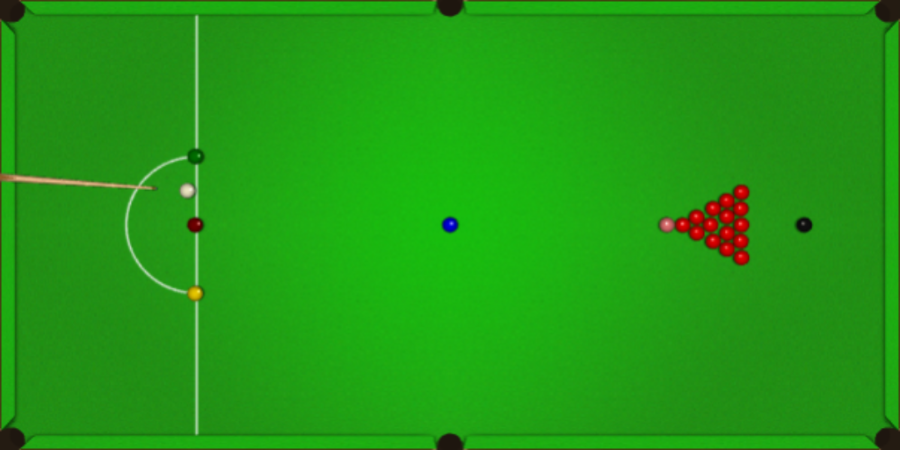
\includegraphics[width=100mm, keepaspectratio]{figures/starting_position.png}
    \caption{A golyók kezdeti pozíciója.}
    \label{fig:kezdeti_pozicio}
\end{figure}

\section{Pontszerzés}
A játékosok a pontjaikat a golyók bizonyos sorrendben való zsebbe helyezésével szerzik. Az egymás után hiba nélkül szerzett pontok összegét \textbf{törésnek} nevezzük. Egy játékos például szerzhet 9 pontos törést a következő golyók egymás utáni elhelyezésével \textit{piros -> zöld -> piros -> barna}.\cite{shamos2002new}
\par Egy játékos büntetőpontokat kap hibák elkövetése esetén. Hibát elkövetni lehet például a fehér golyó zsebbe helyezésével, nem megfelelő színű golyó elütésével. Az elkövetett hibáért minimum 4, maximum 7 pontlevonás jár, attól függően, hogy milyen színű golyók mozdulnak a hiba elkövetésekor (pl.: Ha a cél a piros golyó lelökése, de a lövő a feketét találja el, akkor 7 hibapont jár). A hibát elkövető játékos a törésének pontjait megkapja a hibát elkövetett lövés közben elhelyezett golyók pontjainak kivételével.\cite{snooker_rules}